\chapter{Details}
% ------------------------------------------------------------------------------
% Elaboration 20 pages. Details of the Dependency Analysis Plugin (DAP. Describe
% the DAP-DB and %DAP-INCQUERY solution too.
% ------------------------------------------------------------------------------


\section{Infrastructure at CERN controls systems}

% Eclipse
At CERN Controls group has a definite set of tools used for development. Because
C/C++ and Java applications are developed, the used Integrated Development
Environment is an internally maintained Eclipse distribution with correct
plugins installed.

% SVN, JIRA, Bamboo
To maintain concurrent versions of the source code an SVN server is used. Also
there are a variety of tools used for typical developments tasks: issue
tracking, continuous integration, source code browsing, static code analysis,
etc. 

% Common Build
The central element for the development is a tool called \tool{Common Build}
\cite{CommonBuild}. It is a build and release tool for Java softwares. Common
Build is an Apache Ant based software similar to Maven. It provides
functionality to describe and resolve dependencies, build, generate
documentation and release the softwares. This tool was developed before the
first version of complex build systems such as Apache Maven was published so 
Common Build remained as an in-house build tool. 

% Common build integration with source and binary repositories
Common build is tightly coupled both to the SVN server and to the binary release
repository as it automates the not just the building but the release of the
Java products too.

% Development workflow
\picseventy{commonbuild.pdf}{Build workflow using Common Build}
\autoref{fig:commonbuild.pdf} highlights this relationship by showing a typical
workflow of the development process. The developer first checks out the source
code from the SVN repository and starts working on it. Along source code
modification there is an XML descriptor containing the information required by
Common Build (such as name and version of the product and the required
dependencies). Also Common Build is capable to setup build path and the related
options for Eclipse development. 

% building
When the source code is ready, the developer executes the Common Build client to
build it. The client itself is a customized Ant distribution and acts in the
same way. It resolves the dependencies from the dedicated binary repository
which contains all previously released products and all used third party
libraries. The content is also defined in a XML file.

% release
If all source code is ready the developer can hit release. This fist initiates
the same build process, but it is extended by two things. First the source code
is tagged in the SVN repository which the version number as tag name. Second the
compiled jar file is put into the binary repository. 

% ------------------------------------------------------------------------------
% MODULE: Bytecode analysis
% ------------------------------------------------------------------------------
\section{Bytecode analyzer}
% Why
Before the system performs dependency analysis, it needs to extract the
necessary information from the source code.
% What
The Bytecode analyzer module takes the input java binaries (in the form of jar
files) parses the contained class files with the help of Apache BCEL and maps it
into an object graph which can be effectively used during the dependency
processing.


% How
\subsection{Anatomy of a Java binary}
The Bytecode analyzer module takes a set of jars as an input. A jar file is
essentially a zip file containing Java-related resources: resource files, binary
class files and meta-information. Because the system has to discover
dependencies between pure Java applications then no meta-information is used;
the bytecode analyzer gets the information from the class files contained in the
jars.
 

% Describe the ConstantMethodRef/FieldRef/Class/String in more details?
Figure \autoref{fig:classfile.pdf} shows a simplified view how a single class
file is built. This structure is precisely defined in Java Runtime
Specification. The class begins with a marker header followed by the part called
\textit{constant pool} which contains the textual part of the code. It contains
the i) constant strings ii) referenced methods and fields and iii) the names of
the external classes. The Java virtual machine is only able to load a class file
if all the referenced external classes are loaded.
%\pic{classfile.pdf}{Internal structure of a class file}
After the constant pool the access flags, the implemented interfaces and the
field list are located in separate places.

% Describe the bytecode instructions?
Afterwards comes the definition of the methods. It contains all the necessary
information for the virtual machine to execute the methods: the resources to 
allocate for the execution, the exception handlers and the bytecode itself. 

The big question is what information can be extracted from the jar/class files
for the dependency analysis? The short answer is everything. The structure of a
class file can be obtained one-by-one. The external references what we are
looking for are also fairly easily to extract, because they are defined in the
constant pool. The only challenging part to solve is to match, where exactly are
the external resources are used in the bytecode itself.


\subsection{The analysis process}
The module extract all necessary information from the class files for processing
them. This could be done by brute-force parsing binary files, but it would be an
tedious and error-prone task. Instead of this the implementation reuses Apache
BCEL to effectively parse the class files and and to obtain the necessary
information via simple API calls.
\pic{bytecodeanal.pdf}{Steps of the bytecode analysis process}
\autoref{fig:bytecodeanal.pdf} shows the steps of the analysis process and the
related information in the class files for each step. 

The analysis starts with gathering the basic structure. This involves acquiring
the class' name, the name of the extended class and the implemented interfaces,
the defined fields and methods. This information is accessible out of the box
through the BCEL API.  

The second step is to acquire all external reference pointing outside of the
class files. For imported classes it is easy because this is what the
\code{ConstantClass} entries cover in the constant pool. For field and method
references, the implementations searches \code{ConstantFieldRef} and
\code{ConstantMethodRef} occurrences in the bytecode and saves all methods 
which uses them.

The next step is to convert the information into source format. This is
necessary because both the structure and the external references are presented
in a format which not readable nor could be easily queried by the users of the
data. For example the commonly used \code{println(String)} function has the
following binary format: \code{println(Ljava/lang/String;)V}. The implementation
transforms it into \code{println(java.lang.String):void}.

% Somewhere it should be described that we don't deal with reflection, just
% static dependencies.
The final step is to clean up the gathered information. At this step we have to
consider that if we mapped all information then the gathered data would have a
comparable size with the binary repositories which is unacceptable when we have
to deal with thousands of jars. To resolve this, the implementation does
multiple cleanup steps. First it drops the private methods and fields, because
it is not explicitly accessible and by this no dependency would point them. The
other trick is to drop a subset of the external references. The
platform-provided elements are dropped (references pointing inside the
\code{java.*} package) and the ones which point inside the jar files. This is
reasonable because any IDE gives access this information through code traversal
capabilities. Of course this cleanup needs do be done after all class files are 
parsed in a jar file. 


\subsection{Extracted domain model}
The output of the analyzer is a java domain model.
\picr{domainmodelsimp.pdf}{Classes of the domain model used by the bytecode analyzer}
\autoref{fig:domainmodelsimp.pdf} shows the elements of this model. Because this
model is used for the dependency processing too the model has additional
elements which is now not important.

All element inherits from abstract \code{CodeElement} class which is a top-level
interface for handing the items of the model. The processed jar files are named
as \code{Product}s, because that's what it is: a software product. A product
contains several classes named \code{ApiClass} which store the class-level
properties. The required classes are stored in the \code{referencedClasses}
list. The classes contain some \code{Field}s and some \code{Method}s which both
have a -- source formatted -- signature and some access properties. The
\code{referencedFields} and the \code{referencedMethods} hold all the external
field and method references which are accessed or invoked in the bytecode of the
represented method.

With an instance of this domain model the dependency processing module is
capable of discovering the dependency relationships between certain parts of the
dependency.
 

% ------------------------------------------------------------------------------
% MODULE: Dependeney processor
% ------------------------------------------------------------------------------
\section{Dependency processor}
% Why
The bytecode analyzer gathers all structural elements and the textual references
of the dependencies. For resolving the references the dependency processor
component is responsible.

% What
To achieve this the processor takes the models of the jar files, compares the
contained references with the structure of the external jars. When a match is
found it means that there is a dependency between a two elements and as a result
a dependency is stored.

% How
\subsection{Discovered dependencies}
During the work at CERN we decided to narrow down the search for basic
dependencies which could be extracted from the binary code without interpreting
what does a class really do. By this we could exactly define what information
will be accessible for the users. The following list contains the discovered
dependencies:
\begin{description}
\item[Class import] When a class uses \emph{any} part of an external class. 
Practically this is a relationship between two classes when one class requires
the other to get loaded in the Java virtual machine. On a binary level it is 
expressed as a \code{ConstantClass} entry in the constant pool.  
\item[Inheritance] When a class inherits from another. This dependency type 
covers both the case when an interface is implemented and when a class is 
extended. 
\item[Method call] When a method calls an another method. Covers both static 
and non-static method calls.
\item[Method override] When a class extends from an another and the subclass 
has a method with a same signature which was already defined in the superclass.  
\item[Field access] When a method accesses or gives a value of a field defined 
in an external class.
\end{description}


\subsection{Discovery process}
After defining the searched dependencies let's see how exactly the dependency
discovery process work. The main objective here is to do the analysis on a large
set of Java binaries without having memory problems. Obviously if one loads all
jars at the same to the memory and searches for all references it will need an
enormous size of memory which will go up if the input number of the binaries
increasing.

\picr{analization.pdf}{Sequence of the dependency discovery process}
\autoref{fig:analization.pdf} shows how the tool solves this issue. The process
starts with an update in the binary repository. The new, not analyzed binaries
are passed to the bytecode analyzer components which produces a model for each
jar files. These models passed for the dependency processor which stores the jar
structure in the database. By doing this the implementation holds only one model
in the memory which implies that the memory requirement is independent from the
number of input binaries. Also only the structure is pushed into the database,
the references are considered as transient data. This is necessary because the
references need huge space to store: on average they took 60\% of the size of a
class file and leaving them out is a big saving in the storage.
 
After all jar's  structure is saved in the database, the process re-initiates
the bytecode analysis on every jars one-by one and passes the models again to
the dependency processor. The processor now tries to execute certain queries on
the database for searching dependencies. For external references it tries to
find the elements with the same fully qualified, for inheritance searches for
superclass in the database and for method override it looks for methods with
the same signature in the superclass. Every found element from the database 
result in a dependency entry at the end of the analysis of the current jar. 

The result of the analysis is a database containing all the structure
and the dependency information. The clients execute queries on it to analyze the
relationships between certain elements in order to decide whether or not a
specific code could be changed.
 
 
\section{Storage engine} 
The dependency processing requires some database functionality to 
properly work. This is defined in the storage engine component.

Although this component is defined by a single Java interface it comes with
important and complex responsibilities. First it is an abstraction layer over
the concrete database implementation. Second it provides transactional behavior
automatically to the database. 

The interface defines operations for two purposes: i) Store and retrieve the
structure of a jar and the dependencies ii) search for items based on their
names and iii) query incoming dependencies of an element.

The usage of the first is easy the understand: if the analyze process starts it
has to be checked if the a jar is in the database and if not, it has to be
stored. The second in the list is part of the dependency processing. It is the
responsibility of the database component how to represent the data and thus
finding references also belongs here. The last part covers the queries which are
initiated by the clients and the result is also provided by this module.

To make the domain model usable to store dependencies and make it work with the
same jar products with multiple versions some additions were added (see
\autoref{fig:domainmodelext.pdf}). \pic{domainmodelext.pdf}{Additions to the
domain model} Every element has a list of version numbers where they are
present. Also a \code{Dependency} class is added to effectively handle
dependencies between them.

% emf and oracle implementation.
This database engine is just a specification how it should work. It has two
practical implementation: one which uses Oracle database and one which stores
the data in an EMF model. The Oracle database maps the entities into tables and
execute complex SQL queries in order to find the desired elements.

The EMF version is an in-memory implementation with an optional serialization
feature implemented. The EMF metamodel used for creating the model has the same
structure as the domain model (see \autoref{fig:domainmodelsimp.pdf} and
\autoref{fig:domainmodelext.pdf}).

% TODO: maybe the explanation of the two deps implementation would be fine to
% show here


% ------------------------------------------------------------------------------
% MODULE: Dependeney processor
% ------------------------------------------------------------------------------
\section{Dependency database synchronizer}
% what
The Dependency database component is responsible for querying the server for
dependency information related to a selected element or elements. It loads the
sub-part of the dependency data stored by the storage engine module through a
simple RMI interface and pushes it to the model queries components where the
result is evaluated.
% why: TODO

The component has to inputs: either it can load a compacted representation of the 
entire dependency model or it can query the incoming dependencies for just one 
single code element. 

The single element query is the use-case where the user of the \ptool  executes
direct queries by asking the incoming dependencies of one element in
the workspace. In this case a simple RMI interface method is called where the
argument is the queried object (as an instance of a ApiClass, a Method or a
Field types from \autoref{fig:domainmodelsimp.pdf}. This argument is passed to
the server, which turns it into an SQL query or a search on the EMF model
(depending which back-end is loaded). The result is passed back as a collection
of \code{Dependency} instances. The result model is unattached by the model
queries component and gets instantly visualized in the UI component.

For letting the model queries component run real queries, this model has to load
a representation of the data stored by the database engine component. If it was
loaded one-by-one into an EMF model and passed to the client, then it would be
simply too big to load. The binary repository holds more than a thousand jars
just as latest production versions. The serialized EMF model equivalent is more
than 400 MiB in size. To load an EMF model this size, more than one GiB  of
RAM is needed.

Important details about the environment at CERN is that the developers usually
do the development on dedicated virtual machines which have more privileges to
access internal resources. The drawback is that usually a virtual machine has
1-2 GiB RAM total, so we cannot make an Eclipse plugin which consumes all
remaining resources at once. Also EMF-IncQuery has a practical limitation as it
can easily handle EMF instance models up to 100 MiB.

These facts implied that the repository model has to be compacted. We can drop
the unnecessary information or merge certain data and structure to spare some
space without introducing false negative results. If we leave information the
clients may end up false conclusions as they for example see an empty incoming
dependency set where should be some. 

Sure this compacting process introduces some false-positive results, but in 
return lets the model queries component to do super-fast model queries which
are automatically updated every time the source code has changed. 

The structure of the compacted EMF model is shown on \autoref{fig:cp3model.pdf}.
\picseventy{cp3model.pdf}{Compacted repository model}
The first thing which was left out are most of the fields of the classes; only a
\code{name} field stores the textual representation of the code element. This is
reasonable because the dependency discovery is done on the server and we
navigate only on the dependency edges. The second thing is not explicitly
visible on the figure. The fully qualified name was merged down into simple
names. It means that there is only one \code{Service} class for all products in
the repository and one \code{newService()} function. If there are more than one
exist, they are merged into one and also all dependencies becomes common. This
also comes with the change that the original one-to-many containment
relationships became many-to-many. The third compacting change is to drop the
signature of the methods, only the name has left. The merging process is the
same as described.

% TODO: this should be replaced with true slicing
This compacted repository model is loaded at start-up time and used till Eclipse
is closed. This is reasonable because the repository is not a rapidly changing
entity. Only a few elements are modified each day. Apart from that it wouldn't
be hard to implement a model eviction mechanism, where a new repository model is
loaded every time when somebody does a change in the repository. Luckily this 
wouldn't change anything in the results of this paper.  

\paragraph{}
The described compact model sadly contains some simplification but small enough to
load it into the memory: the serialized representation of the entire workspace is
around 70 MiB which is considered small enough to work with. 

% ------------------------------------------------------------------------------
% MODULE: Source code model synchronizer
% ------------------------------------------------------------------------------
\section{Source code model synchronizer}
% what
To make the repository model comparable with the state of the workspace the
source code model synchronizer generates an EMF model describing the elements
in the workspace and keeps it synchronized along every workspace modification.
Maintaining an EMF model lets the model queries component dynamically examine
the current state of the workspace without accessing the JDT API.

\subsection{Eclipse Java Model}
Eclipse Java Development Tools main objective is to give feature-rich,
integrated and extendable environment for editing Java source code. It comes
with incremental builder and rich and extensive tooling for Java editing.
Contributors can get all the necessary information about the state of the
workspace.

The state of the Java projects are exposed through an API called \emph{Java
Model}. It is a complex yet intuitive set of Java interfaces which can be
traversed easily. Instead explaining what classes and interfaces are present in
this API, let's examine which API elements represents which Eclipse- and
Java-specific elements.
\begin{figure} 
        \centering
        \begin{subfigure}[b]{0.5\textwidth}
                \centering
                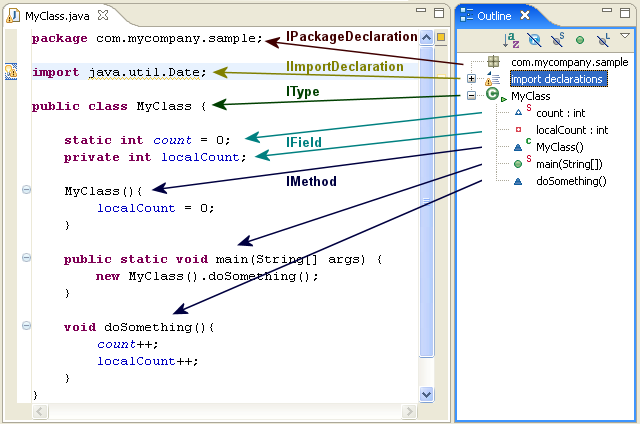
\includegraphics[width=\textwidth]{figures/javamodel2.png}
                \caption{Java Model elements from the source code}
                \label{fig:javamodel2.png}
        \end{subfigure}~
        \begin{subfigure}[b]{0.5\textwidth}
                \centering
                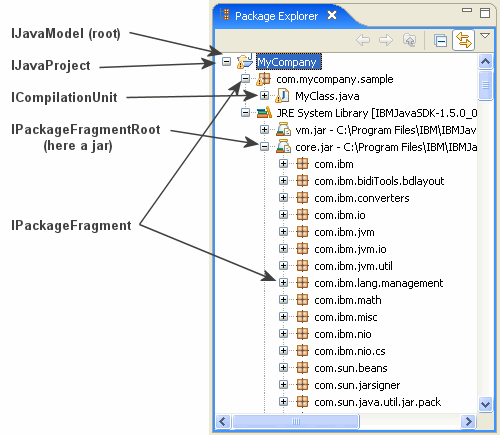
\includegraphics[width=\textwidth]{figures/javamodel1.png}
                \caption{Java Model elements from the navigator}
                \label{fig:javamodel1.png}
        \end{subfigure}
        \caption{Java Model elements}\label{fig:javamodel}
\end{figure}
\autoref{fig:javamodel} (which comes from JDT's documentation) shows these
relationships as the main elements of the Java model. Visible: literally every aspect 
is accessible from the defined projects down to the method level. As the Java Model 
is hierarchical the implementation simply traverses it to build the java model. 

The elements explained above is enough to create a model about the structure of
the Java projects. To add dependency information to this model, the JDT's search
feature comes into picture. With this the component is able to query the dependencies
for every structural element. 

\subsection{The generated EMF model}
% structure and JDT
\picr{wsmodel.pdf}{EMF model storing the structure of the Java projects}
\autoref{fig:wsmodel.pdf} shows the EMF model which is extracted and maintained
from from the Java Model. It mostly mirrors the structure of the Java model's
interface structure. The key element is the \code{WNamedElement} which is common
superclass for all items. The \code{handler} property holds an identifier string
which uniquely identifies the represented Java Model object. To gain access to
the correspondent Java Model object, only the \code{JavaCore.create(String)} is
required.

% structural hierarchy.
The containment hierarchy starts form the lower right corner of the figure with
the \code{WProject} class which represents a Java project loaded into the
workspace. It contains \code{WPackageFragmentRoot} elements which represent the
source folders and the jar files on the classpath and has some Java packages as
children(as \code{WPackageFragment} instances). Under the Java packages there
are the \code{WCompilationUnit}s which are represent the java files and which
define some java types (\code{WType}). On the lowest level in the containment
hierarchy lie the methods and fields (\code{WMethod} and \code{WField}
instances).

% dependency hierarchy.
Just like in the repository model here also the dependencies are defined upon
the common supertype, but here a \code{WDependency} has a two-way relationships
for both the source and the target part of the dependency relation. For one
\code{WNamedElement} the incoming and outgoing dependencies are directly
accessible. Again, the same dependency types are defined as before.

% root
The model has one common root, a \code{WWorkspace} instance which contains both
the structural elements and the dependencies.

\subsection{The model synchronization process}
% describe the process itself
\picr{sourcesync.pdf}{The maintenance process of the source code model}
\autoref{fig:sourcesync.pdf} shows how the process  of model building works. It
starts with mapping the entire workspace structure (projects, classes, etc.)
into the model. During the process the entire workspace is traversed. If it is 
done the components executes a dependency search for each relevant element 
utilizing JDT's integrated search engine. The found dependencies are associated 
with the proper model element.

When the initial model build is finished the next task is to subscribe for the
workspace changes. This can be done by registering a simple listener object with
the  \code{JavaCore.addElementChangedListener(IElementChangedListener);} static
method. With this every event related to the java editing is available. The
component only handles the events where the source files are changed; dealing
with working copy events would be too frequent and would contain some incoherent
data about the workspace. 
	
After the component is set up it waits for the modifications. If it happens, an
incremental model update fires, maps the related Java Model element to the EMF
model and modifies it properly. 

The change notifications comes in a form of a hierarchical delta holder object.
It refers to an object, states if it was added, deleted, or changed and provides
the list of the affected children. For example if a Java class definition has
been deleted, the generated event contains a changed project down to the
container changed compilation unit which has a child delta pointing to the
deleted class.

The use-case when an element was added or deleted the model update is
straightforward. The event contains the reference of the modified item. It is
identified via the \code{handler} property. The result of the event is a
creation of a new element or removing an existing one along with all his
children and their dependencies.

If a modification happens in the source file it is also incrementally modified
but treated slightly differently. This is necessary because the delta
information doesn't provide usable information about what has changed below the
compilation unit.
\pic{sourceupdate.pdf}{Updating EMF workspace model when source code is modified}
This process is shown in \autoref{fig:sourceupdate.pdf}. The updater checks
which source file is modified and re-generates its EMF representation. The
generated small model is compared with the source of the model. If a new method
is added than it is merged into the old model. If an element is missing, it gets
deleted from the original model too. Dependencies are the same: any differences
are immediately pushed back to the original model. With this approach the EMF
representation of the workspace stays consistent and only local modifications
happen on the elements.

When Eclipse closes, the model is stored on the disk in order not to regenerate
the entire model when on the next start-up. If no external modifications happen
than the model is loaded one-by-one which is faster than gathering all
structural and dependency information.

\section{Model queries}
The model queries components executes complex queries on the loaded models and
gives and exposes the result for  visualization. 

Both the result of the explicit queries and the EMF-IncQuery-based use-case is
handled inside this component. As it was discussed previously not much has
happening here with the result of the explicit queries: it is passed to the UI
components as is.

The more interesting part of the module is the queries based on EMF-IncQuery.
The main reason why it was implemented is that normally, if the analysis is done
only on the server side, than all the dependency information will be based on
the released source code. So if a developer changes something and after tries to
figure out what are the dependencies of the changes elements, he won't get any
results. This is why we want to compare the repository with the current state of
the workspace.

Applying this approach will not only give the developers precise information
about the impact a possible release would cause but it gives immediate feedback
about the change every time the source code is saved. Also important that
all results of all queries is available upon usage, no manual query is required.

To achieve this, the component first loads the model of the repository and the 
model of the current workspace, loads them into the EMF-IncQuery engine, 
and initiates the queries and exposes the results on an API which also updates
the dependency information dynamically. 
 
The queries are developed with EMF-IncQuery's own query language. This language
is used to express certain patterns over EMF models. You can think about it as 
a regular expression over an object-model. To highlight this, let's see an example
of a pattern expressed with this language which matches on all Java files and
all defined types in it from the workspace model (see \autoref{fig:wsmodel.pdf}). 
\begin{lstlisting}
package example

import "http://inf.mit.bme.hu/donat/incquery-deps/wsmodel"

pattern typesInJavaFiles(cu : WCompilationUnit, t : WType) = {
	WCompilationUnit(cu);
	WType(t);
	WCompilationUnit.types(cu, t);
}
\end{lstlisting}

The import declaration loads the schema of the EMF moel. The pattern signature
contains a name and a parameter list. Here the parameters define the result as
the found/matched items from the input model. 

The body of the pattern starts with two type constraints. This can be translated
as ''match only on the elements which have the \code{WCompilationUnit} type for
the \code{cu} variable and match the \code{WType} object for \code{t}
variable''. Alone this would list all compilation units and all types as a
result in all possible combinations, just like in SQL when one select data from
two different tables at once without joining them. The third statements is the
connects the result items together. It can be translated as ''match only the on
the objects  where the \code{cu} variable references the \code{t} as a contained
type''. Expression power of the pattern language is much bigger; for complete
reference check the documentation site \cite{EMFIncQuery}.

The usage of the queries takes multiple steps shown on \autoref{fig:incquerydev.pdf}.
\picr{incquerydev.pdf}{Development of EMF-IncQuery queries} 
First the queries are defined with the query language. The tooling takes the queries 
and automatically generates source code from the queries. With this there is no need 
for manually using the pattern definition part of the EMF-IncQuery engine. The generated
source code along with the engine exposes a simple interface for registering the
queries and getting back the results when needed. The only manual coding takes place
at the last part on load-time, when it has to be specified manually which queries 
should be evaluated. 
  
The generated code contains a factory service which registers the query in the
engine. The query is represented as a \code{Matcher} object in the generated
code which gives back the results through the \code{Matcher.getAllMatches()}
method. The result is represented by \code{Match} instances which hold the result 
and all the necessary information to make it usable.

The following list enumerates all the  queries developed for the dependency
analysis.
\begin{description}	
\item[Join queries]
In order to compare the workspace with the repository it is necessary to find 
the correspondent element in the two model. The join queries are basic patterns 
which joins the projects, classes, fields and methods in the models. The result
of the queries are all the found elements which are the input for the queries 
below. 
\item[Workspace changes] These queries discover the differences between the 
workspace and the repository. The results are the projects, classes, methods
and fields added or removed from the source code.   
\item[Incoming dependencies] For every source code loaded in the Eclipse these
queries shows all elements depending  on them. All incoming dependencies for 
all classes methods and fields are the result of these queries. Also the type
of the dependency is available. 
\item[Outgoing dependencies] The queries in this category can be highlighted 
with the following: If a dependency exists in the workspace it should
exist in the repository too. If the workspace changes and the dependencies change
it can be source of the problem.  By checking the changed outgoing dependencies
which start form the selected items the developer can analyze it.
\item[Commit impact] This list contains queries which are the combination of 
the workspace changes and incoming dependencies category. They show the incoming
dependencies of items which have changed in the workspace. The result is the
impact which a possible release would cause.  One use-case is to show the
incoming dependencies of the deleted elements. Another can be inheritance on
the classes where a method is added.
\end{description}

On start-up these queries are registered and accessible outside via a simple API.
The UI components use this API to access the dependency information and show the
current state in different views.

\section{UI Components}
Eclipse UI contributions provide the way to access to the input and the output of \ptool . 
These elements are grouped into in this component. 

UI for direct queries
First: contributions to the source code editor. 
Context menu gets new item: show incoming dependencies.
Finds selected element and executes dependency query. 
The query contains a fully qualification, then sends the actual request and waits for the result.
When it is sent, the result is provided in an Eclipse view.

Alse Eclipse views are used to display the result  from the EMF-IncQuery engine.
Using JFace has two advangage: the style of display is not bound to the data EMF
technology has out of the box integration with jface.

insert picture from diagram-source.
Query result is restructured into an own tree-like structure.
An adapter object is created. It makes JFace understand how to interpet
the obtained data.

The explicit queries does not require any change listener because it alwasy show
one query information.
However the EMF-IncQuery shows dinamic data so the view is updated dinamically
View registers itself to the Eclipse platform selection service and updates the
relevant information automatically as the selection changes. 



